%% CAPITULO 2
\hypertarget{estilo:capitulo}{}
\chapter{DADOS E METODOLOGIA}

\section{Dados}
\label{ss:dados}

Para o período de estudo este trabalho, foram utilizados dados observados de precipitação provenientes de estações de superfície e dados estimados de satélites meteorológicos. Estes dados foram utilizados para a elaboração dos campos iniciais de precipitação, utilizados na assimilação pelo modelo Eta e na avaliação dos resultados. Adicionalmente dados das reanalises do CPTEC e do NCEP/DOE foram utilizados também para comparações e verificações do desempenho do sistema Eta+RPSAS com e sem a inclusão da precipitação estimada. Nos tópicos a seguir, apresenta-se uma breve descrição desses conjuntos de dados.

\subsubsection{\textit{Tropical Rainfall Measuring Mission} (TRMM)}

O satélite TRMM foi lançado em 27 de novembro de 1997 e é um projeto de parceria entre a NASA e a Japan Aerospace eXploration Agency (JAXA), tendo como missão principal  fornecer informações sobre a estrutura e a distribuição espacial da precipitação, sua influência no clima das regiões tropical e subtropical e sua importância no ciclo hidrológico (SIMPSON et al., 1988, 1996).

O TRMM possui órbita polar com 35° de inclinação a 380 km de altura, com alta resolução temporal (possui um período de translação de apenas aproximadamente 90 minutos e 16 órbitas por dia) varrendo as faixas de latitudes tropicais (50°N e 50°S). Além disso, o TRMM é equipado com sensores específicos para o estudo da precipitação possibilitando a aquisição de informações sobre a precipitação tropical, relâmpagos e sobre a energia radiante das nuvens e da superfície terrestre. Estes sensores incluem:

\begin{itemize}
\item Imageador de microondas (TMI);
\item Radar de precipitação (PR);
\item Radiômetro no visível e no infravermelho (VIRS);
\item Sensor de energia radiante da superfície terrestre e das nuvens (CERES);
\item Sensor para imageamento de relâmpagos (LIS).
\end{itemize}
    
Além disso, as estimativas de precipitação são validadas em superfície através de um programa em paralelo denomidano \textit{Groud Validadtion} (GV) que conta com uma série de radares meteorológicos em superfície espalhados ao longo da faixa intertropical \cite{collischonnetal07}. 

Os dados estimados de precipitação provenientes do TRMM, que foram utilizados nos experimentos de assimilação deste trabalho, possuem resolução horizontal de 0.25° de latitude/longitude e frequência temporal de 1 hora. As estimativas de precipitação calculadas pelo TRMM são obtidas a partir do algoritmo 3B42, utilizando informações sobre a estrutura vertical das nuvens.
    
O algoritmo 3B42 é uma combinação de estimativas de precipitação por microondas e infravermelho corrigidas através das informações sobre a estrutura vertival das nuvens, obtidas pelo radar de precipitação a bordo do satélite. O algoritmo para o cálculo das estimativas segue os seguintes passos:

\begin{enumerate}
\item Estima-se a precipitação com informações de dados de microondas (TMI); 
\item Estima-se a precipitação com informações do canal infravermelho (VIRS); 
\item Calibra-se a precipitação estimada por microondas e por infravermelho, disponibilizando-se as estimativas finais de precipitação a cada hora.
\end{enumerate}

\subsubsection{\textit{South America Low Level Jet EXperiment} (SALLJEX)}

O South American Low-Level Jet EXperiment (SALLJEX) é um experimento de campo iniciado no centro-oeste da AS durante o período de 15 de novembro de 2002 a 14 de fevereiro de 2003 (VERA, 2006; HERDIES et al. 2007). O programa South American Low-Level Jet (SALLJ), um componente do programa Climate Variability and Predictability/Variabilty of the American Monsoon Systems (CLIVAR/VAMOS), em linhas gerais, é um esforço coordenado internacionalmente para uma maior compreensão do papel que os JBN desempenham sobre a AS no transporte de umidade e nas trocas de energia entre os trópicos e extratrópicos, além da caracterização de aspectos da hidrologia regional, clima e variabilidade climática para a região de monção da AS (HERDIES et al., 2007). 

Durante a campanha, uma grande rede de pluviômetros foi instalada, além de 6 estações provisórias de ar superior e 16 novas estações de balão piloto no Peru, Bolívia, Paraguai, Argentina e Brasil. A Figura 8 mostra a distribuição espacial das radiossondagens e dos balões-piloto utilizados durante o período de estudos do SALLJEX na AS. As informações providas pelo experimento são de grande importância para a execução do presente trabalho, pois representam dados de superfície e de radiossondagem (com 1º de resolução espacial) que serão utilizados para a avaliação dos processos de assimilação com o sistema de assimilação de dados RPSAS do CPTEC.

\begin{figure}[!hbp]
\includegraphics[height=8cm]{./figs/salljex.png}
\caption{À esquerda, distribuição espacial dos pontos de coleta de dados meteorológicos do SALLJEX. As radiossondagens são representadas pelos quadrados e, os balões-piloto, pelos círculos. Em sombreado é apresentada a topografia do modelo global com resolução de aproximadamente 100 Km. Fonte: Herdies et al., 2007. À direita, rede de radiossondas do experimento SALLJ. Fonte: Adaptado de Zipser et al., 2004.}
\FONTE{à esquerda: \citeonline{herdiesetal07}; à direita: adaptado de \citeonline{zipseretal04}}
\label{fig06}
\end{figure}

\subsubsection{Reanálise Regional CPTEC}

Para a comparação dos resultados obtidos a partir das simulações, foram utilizados os campos atmosféricos da reanálise do CPTEC (ARAVÉQUIA et al., 2007) para o período do SALLJEX. A reanálise do CPTEC foi gerada com o sistema de assimilação de dados RPSAS com 40 km de resolução espacial e 38 níveis verticais (versão 2003) e cobre o período de 2000 a 2004. Como condições de contorno, foram utilizadas as análises operacionais do modelo global do NCEP (T62L28). 

Estes dados de reanálise são a combinação de dados observados com modelagem numérica e representam o estado da atmosfera mais próximo da observação para o período de estudos sobre a AS. O conjunto de análises da reanálise de 40 km do CPTEC inclui perfis recuperados de temperatura e umidade (provenientes do ATOVS), dados de vento de satélites (CTW e Quickscat), dados convencionais de superfície (SYNOP e BUOY) além de dados de sondagens dos experimentos RACCI-LBA/2002 (Silva Dias et al., 2003) e SALLJEX. Como produtos da reanálise do CPTEC, foram obtidas análises dos campos meteorológicos de variáveis comuns (prognosticadas e diagnosticadas pelo modelo Eta – ventos, temperatura, umidade, cobertura de nuvens etc), além de subprodutos espaciais, tais como campos climatológicos, médias diárias e mensais, precipitação diária, temperaturas máxima e mínimas entre outros.

\subsubsection{Reanálise Global NCEP}

A Reanálise 2 do NCEP/DOE (KANAMITSU, 2002) é a versão corrigida da Reanálise 1 do NCAR (KALNAY, 1996) que tem como objetivo introduzir melhorias e correções. A Reanálise 2 do NCEP/DOE foi construída utilizando-se o modelo global T62L28 do NCEP e cobre o período de 1979 a 2009, tendo-se como meta expandir-se até 1950. Os dados da reanálise 2 do NCEP tem como principal objetivo fornecer informações mais acuradas sobre o passado utilizando dados de observação e modelagem numérica. As principais vantagens em se utilizar esta nova versão da reanálise em relação à sua versão anterior está na melhor representação do ciclo hidrológico, campos aprimorados de umidade do solo e temperatura à superfície, precipitação, cobertura de neve e outro.

Em Kanamitsu (2002) estão enumerados alguns defeitos/erros (erros de programação) cometidos durante o processo de obtenção da reanálise. Dentre eles, destacam-se os seguintes, por serem correlatos à algumas variáveis avaliadas neste trabalho de dissertação: erros de correção da umidade do solo quando este está saturado (ao invés de aplicar a correção de saturação do solo à segunda camada, esta foi aplicada à primeira); erros na redução da umidade do solo em casos em que a precipitação do modelo (ou ainda o run-off do modelo) é menor do que a precipitação observada.

\section{Metodologia}
\label{ss:metodologia}

O Ciclo de Assimilação de Dados (CAD) do Centro de Previsão de Tempo e Estudos Climáticos (CPTEC) utilizado neste trabalho é composto de dois  componentes essenciais: o Controle de Qualidade (CQ) e o sistema regional de assimilação de dados RPSAS. A seguir é dada uma descrição sucinta destes dois componentes.

\textbf{a) Controle de Qualidade}

Nesta fase é realizada uma depuração dos dados (observações) provenientes do \textit{Global Telecommunicatio System} (GTS) e de diversas outras fontes tais como o \textit{Internet Data Distribuition} (IDD), a Divisão de Satélites e Sistemas Ambientais (DSA/CPTEC), cooperações diretas com agencias espaciais e outros.

A checagem do controle de qualidade é feita em duas etapas: a primeira que abrange o desvio da observação em relação ao mesmo ponto dentro do campo de \textit{first guess} (que é denominado de \textit{background check}) e a segunda que aborda a consistência da observação em relação à sua vizinhança (denominada de \textit{buddy check}). No \textit{background check} as observações são rejeitadas ou assimiladas segundo um nível de tolerância determinado a partir das estatísticas de erro prescritas pelo sistema de análise. Caso o valor trazido pela observação esteja acima do nível tolerável, esta observação é rejeitada. Caso ele possua um desvio grande, mas dentro do nível de tolerância, essa observação é marcada como “suspeita” e, a partir daí procede-se ao \textit{buddy check}. No caso do sistema PSAS, este controle de qualidade é feito para as observações de ventos (componente zonal e meridional separadamente), altura geopotencial e umidade.

A partir disso, quando as observações são aceitas pelo sistema de assimilação, são calculadas diferenças entre os valores observados e estimados do \textit{first guess}. Estas diferenças são então utilizadas para a correção dos campos de previsão de curto prazo gerando a análise.  Maiores detalhes sobre o controle de qualidade do sistema de assimilação podem ser encontrados em ANDREOLI et al., 2007.

\textbf{b) Sistema de Assimilação de Dados}

A seguir sao descritos de forma resumida os componentes do sistema de assimilação de dados RPSAS e como a é feita a nclusão da precipitação no sistema.

\subsubsection{Análise - \textit{Regional Physical-space Statistical Analysis System} (RPSAS)}

O sistema de assimilação de dados \textit{Regional Physical-space Statistical Analysis System} (RPSAS) é a versão regional desenvolvida e mantida pelo CPTEC em parceria com o \textit{Global Modeling and Assimilation Office} (GMAO) da \textit{National Aeronautics and Space Administration} (NASA). O RPSAS utiliza o mesmo sistema de análise do \textit{Physical-space Statistical Analysis System} (PSAS) (Da SILVA et al., 1995; COHN et al., 1998). O RPSAS é considerado um esquema com características de Interpolação Ótima e de esquema variacional em três dimensões (3DVar), porém com a vantagem de ser independente do modelo não sendo necessária a linearização e a criação de modelos adjuntos para a assimilação (por se tratar de um sistema estatístico). Esse sistema de assimilação é utilizado de forma experimental com 20 km de resolução espacial em conjunto com o modelo regional Eta principalmente para previsões de tempo de curto prazo (até 72 horas). O RPSAS é capaz de utilizar dados convencionais provenientes do GTS, tais como SYNOP, TEMP, SATOB entre outros, além de dados não convencionais de satélite (\textit{QuikSCAT}, TRMM, ATOVS, AIRS etc.). 

O RPSAS utiliza como núcleo de análise o próprio PSAS, sendo que as equações de análise e inovação são resolvidas para o caso regional. Para calcular as inovações trazidas pelas observações e como forma de calcular a análise, são utilizadas as seguintes equações (adaptado de \citeonline{larsonetal98}):

\begin{equation}
(HP^{f}H^{T}+R)X=\textit{\textbf{w}}^o-H\textit{\textbf{w}}^f
\label{form01}
\end{equation}

\begin{equation}
\textit{\textbf{w}}^a-\textit{\textbf{w}}^f=P^{f}H^{T}X
\label{form02}
\end{equation}

Em que:

\begin{equation}
X^{a}=X^{b}+W[y^{o}-H(X^{b})]
\label{form03}
\end{equation}

Onde:

\begin{itemize}
\item $P^{f}$: é a matriz (de ordem $n$) de covariância dos erros da previsão;
\item $R$: é a matriz (de ordem $p$) de covariância dos erros de observação;
\item $H$: é uma matriz de ordem $p$$\times$$n$ que interpola as observações na grade no vetor previsão (em ponto de grade);
\item $\textit{\textbf{w}}^o$: é o vetor das observações, de ordem $p$;
\item $\textit{\textbf{w}}^f$: é o vetor previsão (em ponto de grade), de ordem $n$;
\item $\textit{\textbf{w}}^a$: é o vetor análise, de ordem $n$;
\item $\textit{X}$: é a matriz de covariância dos erros de observação.
\end{itemize}

O lado direito da \autoref{form06} é chamado de Vetor Inovação ou Resíduo Observação Menos Previsão (\textit{Observation Minus Forecast} - OMF), e o lado esquerdo da \autoref{form07} é chamado de Incremento da Análise (AI - Analysis Increment). É importante observar que o PSAS ingere os dados observacionais através do vetor OMF na forma $\textit{\textbf{w}}^o-H\textit{\textbf{w}}^f$.

O PSAS resolve a \autoref{form06} e a \autoref{form07} sem formar explicitamente as matrizes $HP^{f}H^{T}$, $R$ e $P^{f}H^{T}$. A representação destas matrizes e a solução da \autoref{form06} e da \autoref{form07} podem ser encontradas em \citeonline{guoetal98}.

Em termos de custo computacional, como mencionado anteriormente, o PSAS é capaz de realizar os cálculos no ponto em que as observações de encontram. Considerando-se um sistema em que $n=10^{6}$ e $p=10^{5}$ (aproximadamente), arranjando-se e resolvendo-se a \autoref{form06}, o esforço computacional para o PSAS é reduzido pela metade (em relação ao 3DVar). O resto do tempo de máquina é devido à transformação da matriz $X$ (da \autoref{form07}) das observações para o espaço das observações \cite{cohnetal98}.

De forma simplificada, o PSAS segue o seguinte algoritmo:

\begin{enumerate}
\item Construção da matriz $HP^{f}H^{T}+R$ e solução da \autoref{form06} para $X$;
\item Construção da matriz $P^{f}H^{T}$ da \autoref{form07} e cálculo do incremento da análise ($\textit{\textbf{w}}^a-\textit{\textbf{w}}^f$) a partir de $X$;
\item Cálculo da previsão e da matriz dos erros de covariância das observações (matriz $X$) para uso nos passos \textit{a} e \textit{b};
\item Particionamento (tipagem) e outros processamentos nos dados observacionais de entrada.
\end{enumerate}

\subsubsection{Previsão - Modelo de Mesoescala Eta}

O modelo regional Eta (MESINGER et al., 1988; BLACK 1994) utilizado nas simulações é a versão pré-operacional utilizada no CPTEC para PNT com 20 km de resolução horizontal e 38 níveis na vertical. Esta versão do modelo Eta é uma modificação da última versão operacional do NCEP (a partir da qual também originou-se a versão \textit{Workstation}) em que foram implementadas algumas melhorias  e foi escolhida para a realização dos experimentos por ser uma versão mais atual do modelo, que inclui um conjunto de física mais moderno e por ser utilizada com maior resolução. Além disso, esta versão do modelo Eta vem sendo utilizada modo pesquisa junto com o sistema RPSAS há alguns anos pelo grupo de AD do CPTEC, sendo, portanto, uma versão pré-operacional. 

Basicamente, a diferença entre a versão operacional e a versão pré-operacional do modelo está na implementação física, que é mais completa na versão pré-operacional utilizada (outras diferenças a Tabela 1 adiante). De forma geral, o modelo Eta se propõe a prever com detalhes sistemas organizados de mesoescala tais como CCM, Sistemas Frontais, Brisas Marítimas, Tempestades e outros (CHOU, 1996).

Como principais características, esta versão do modelo Eta pode ser utilizada nos modos hidrostático e não hidrostático (quando considera os movimentos verticais) e com uma coordenada verical eta que, em comparação à coordenada sigma, reduz os erros numéricos no cálculo da força do gradiente de pressão nas encostas de topografias íngremes. A Equação \autoref{form04} define a coordenada vertical eta:

\begin{equation}
\eta=\frac{(p-p_{top})}{(p_{s}-p_{top})}\bigg[\frac{p_{ref}(z_{0})-p_{top}}{p_{ref}(z_{s})-p_{top}}\bigg]
\label{form04}
\end{equation}

Onde:

\begin{itemize}
\item $p$: é a pressão;
\item $p_{top}$: é a pressão no topo do modelo;
\item $p_{s}$: é a pressão na superfície;
\item $p_{ref}$: é a pressão de referência sobre uma superfície $\eta$ no topo de uma montanha ($z_{s}$) e na base da mesma ($z_{0}$).
\item $\frac{(p-p_{top})}{p_{s}-p_{top}}=\sigma$ (coordenada sigma)
\end{itemize}

O modelo utiliza uma grade horizontal do tipo semi-alternada E de Arakawa \cite{arakawalamb77} e um esquema de integração temporal \textit{split-explicit} - no qual os modos associados à gravidade são tratados com um passo de tempo menor, 20 km de resolução espacial e 38 níveis verticais, com o topo do modelo a 25 hPa. Para uma melhor simulação dos processos próximos à superfície, o modelo possui 17 níveis verticais entre a superfície e o nível de 700 hPa. O domínio de integração do modelo regional cobre a maior parte da AS e parte dos oceanos Atlântico e Pacífico, aproximadamente entre as latitudes de 10ºN - 60ºS e entre as longitudes de 90ºW - 20ºW (\autoref{fig05}). 

\begin{figure}[!hbp]
\centering
\includegraphics[height=10cm]{./figs/fig05.png}
\caption{Topografia (sombreado colorido) e Domínio (sombreado cinza) de integração do modelo regional EtaWS com resolução horizontal de 20 km.}
\label{fig07}
\end{figure}

Em relação aos processos físicos, o modelo EtaWS possui um conjunto de física completa com parametrizações para precipitação convectiva rasa e profunda. O modelo utiliza o esquema de convecção \textit{Cumulus} Betts-Miller melhorado por Janjić (BMJ) \cite{betts86}, \cite{bettsmiller86}, \cite{janjic94}. 

O esquema BMJ considera apenas movimentos verticais ascendentes (convecção). O movimento convectivo transporta calor e umidade removendo ou reduzindo a condição de instabilidade da atmosfera (quando a atmosfera real é mais ou menos úmida do que a atmosfera de referência) alterando os perfis verticais de calor latente e umidade. A atmosfera de referência considera perfis de temperatura e umidade observados por \citeonline{betts86} e \citeonline{bettsmiller86}, que são relativamente secos e seguem adiabáticas úmidas. O esquema é acionado quando a atmosfera real é mais úmida do que a atmosfera de referência (ambiente condicionalmente instável).

Outro aspecto relevante do modelo EtaWS, é a parametrização de superfície. O esquema de superfície utilizado no EtaWS, inclui o modelo NOAH \textit{Land Surface Modelo} (NOAH LSM - \cite{mitchell01}). Esta versão do NOAH utilizada em conjundo com o modelo EtaWS inclui 16 classes diferentes de solo (entre 0 e 30 cm de profundidade) e 24 classes diferentes de vegetação (\autoref{fig06}). As tabelas com os nomes das classes de solo e vegetação do NOAH LSM podem ser encontrada no Anexo A deste trabalho).

\begin{figure}[!hbp]
\centering
\includegraphics[height=7cm]{./figs/soilveg.png}
\caption{Classes de Solo e Vegetação do Modelo de Superfície NOAH.}
\label{fig08}
\end{figure}

Entre outros aspectos da física do modelo, pode-se citar:

\begin{itemize}
\item \textbf{Dinâmica:} Hidrostática ou Não-Hidrostática - o modelo pode ser executado com a coordenada vertical sendo a pressão ou a altura, respectivamente (nos experimentos, o modelo é ajustado para o modelo não-hidrostático);
\item \textbf{Turbulência:} Mellor-Yamada 2.5 para as trocas verticais na atmosfera livre (entre as camadas do modelo) e Mellor-Yamada 2.0 para as trocas entre a superfície e a camada mais baixa do modelo \cite{melloryamada74};
\item \textbf{Processos radiativos:} Lacis-Hansen para o cálculo da radiação de onda curta \cite{lacishansen74} e Fels-Schwarzkopf para o cálculo da radiação de onda longa \cite{felsschwarzkopf75};
\item \textbf{Nuvens:} esquema de microfísica de nuvens de Ferrier \cite{ferrieretal02}, onde podem ser estimadas nuvens altas, médias e baixas além de diversos tipos de hidrometeoros.
\end{itemize}

A \autoref{tab01} resume as principais diferenças entre a versão operacional do modelo Eta e a versão pré-operacional EtaWS utilizada neste trabalho.

\begin{table}[!hbp]
\caption{Diferenças principais entre os modelos Eta e EtaWS.}
\label{tab01}
\centering
\begin{tabular}{c|c|c|c}
\hline
Característica                       &                         & Eta               & EtaWS              \\
\hline
\multirow{2}{2.8cm}{Dinâmica}        &                         & \multirow{2}{2.8cm}{Hidrostática}      & Hidrostática       \\
                                     &                         &                   & Não-Hidrostática   \\
\hline
                                     & Superfície              & OSU LSM           & NOAH LSM           \\ 
\multirow{2}{2.8cm}{Parametrizações} & Precipitação Convectiva & Betts-Miller      & Betts-Miller-Janjić\\
                                     &                         &                   & Kain-Fritsh        \\
                                     & Microfísica de Nuvens   & Zhao              & Ferrier            \\
\hline
\end{tabular}
\end{table}

O albedo e fração de cobertura vegetal foram obtidos a partir de climatologias globais sazonais e mensais, respectivamente. As condições iniciais ($u$, $v$, $t$, $q$, $p_{s}$ - ventos temperatura, umidade e pressão à superfície) no primeiro ciclo de assimilação foram provenientes da análise do NCEP, e fornecidas posteriormente pelo processo cíclico de assimilação.  As condições de contorno foram geradas pelo modelo global T213L42 do CPTEC e atualizadas a cada 6 horas. A temperatura do mar foi obtida a partir dos valores semanais anteriores ao período de estudo com resolução 1ºx1º e mantida constante durante o período de integração do modelo.


\subsubsection{Assimilação de Precipitação}

No sistema de assimilação Eta+RPSAS foram ajustados os campos de temperatura e umidade do modelo seguindo o método de CAR e BALDWIN (1991) através dos campos de precipitação estimada do TRMM (observada), durante o período da geração do \textit{first guess},  6 horas antes da previsão de 24 horas como está esquematizado na Figura 7. Este processo foi iniciado sempre nos horários 00Z, 06Z, 12Z e 18Z (Figura 6).

\begin{figure}
\centering
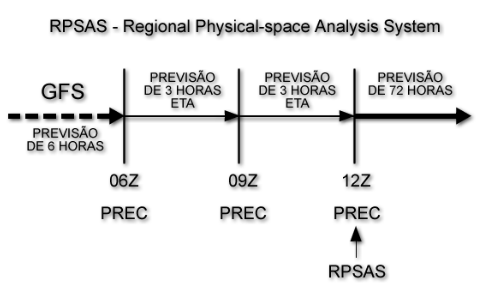
\includegraphics[height=7.5cm]{./figs/rpsas.png}
\caption{Ciclo de assimilação de dados RPSAS/CPTEC para o ciclo de 12Z – \textit{first guess} e análise.}
\label{fig09}
\end{figure}

Os campos de precipitação observados considerados para esta técnica, foram as taxas de precipitação do TRMM, cuja descrição foi apresentada na seção anterior. Este método foi implementado no sistema de assimilação RPSAS por FERNANDEZ (2008), seguindo basicamente o sistema de assimilação de dados EDAS do NCEP.

Para isso, em cada passo de tempo e em cada ponto de grade onde as observações de precipitação estão disponíveis, durante o período de geração do \textit{first guess}, compara-se a precipitação prevista ($P_{mod}$) com a precipitação observada ($P_{obs}$). Com isso, procede-se a uma avaliação da seguinte forma (a \autoref{tab02} resume as condições seguintes):

\begin{table}[!hbp]
\caption{Ajuste convectivo pelo método de Carr e Baldwin adaptado para o \-mo\-de\-lo EtaWS.}
\label{tab02}
\centering
\begin{tabular}{|c|c|c|c|}
\cline{3-4} 
\multicolumn{1}{c}{} &  & \multicolumn{2}{c|}{Ajustes}\tabularnewline
\hline 
\begin{sideways}

\end{sideways} &  & Ajusta-se $P_{mod}$ para 0; & \tabularnewline
\begin{sideways}

\end{sideways} &  & Ajusta-se o perfil de calor & \tabularnewline
\begin{sideways}

\end{sideways} & $P_{obs}=0$ & de acordo com $P_{mod}$; & Não é necessário fazer ajustes\tabularnewline
\begin{sideways}

\end{sideways} &  & Ajusta-se $q_{v}$ de forma que & \tabularnewline
\begin{sideways}

\end{sideways} &  & $RH$ permaneça inalterado. & \tabularnewline
\cline{2-4} 
\multirow{2}{0pt}{\begin{sideways}Condições\end{sideways}}
\begin{sideways}

\end{sideways} &  &  & Especifica-se uma camada\tabularnewline
 
\begin{sideways}

\end{sideways} &  & Multiplica-se o perfil de calor & vertical de nuvem baseada\tabularnewline
\begin{sideways}

\end{sideways} &  & latente do modelo por $\frac{P_{obs}}{P_{mod}}$; & em $P_{obs}>0$;\tabularnewline
\begin{sideways}

\end{sideways} & $P_{obs}>0$&  & Especifica-se um perfil\tabularnewline
\begin{sideways}

\end{sideways} &  & Ajusta-se $q_{v}$ de forma que & parabólico de calor latente;\tabularnewline
\begin{sideways}

\end{sideways} &  & $RH$ permaneça inalterado. & Especifica-se $RH$ na camada\tabularnewline
\begin{sideways}

\end{sideways} &  &  & de nuvem para 80$\sim$90\%.\tabularnewline
\hline
\multicolumn{1}{c}{} &  & $P_{mod}>0$ & $P_{mod}=0$ ou $P_{mod}<<P_{obs}$\tabularnewline
\cline{3-4} 
\multicolumn{1}{c}{} &  & \multicolumn{2}{c|}{Condições}\tabularnewline
\cline{3-4} 
\end{tabular}
\end{table}

\begin{enumerate}
\item Se $P_{mod}>0$ e $P_{obs}=0$: toma-se novamente $P_{mod}$ e a quantidade correspondente de calor latente do modelo; ajusta-se a razão de mistura do vapor d'água ($q_{v}$) de forma que a umidade relativa ($RH$) permaneça inalterada; reduz-se a razão de mistura do vapor d'água para um valor além do necessário a fim de se proporcionar condições para produzir chuva ($q_{cmin}$);
\item Se $P_{mod}>P_{obs}>0$: reduz-se a liberação de calor latente em cada camada de precipitação através da multiplicação do perfil de calor latente pelo fator $\frac{P_{obs}}{P_{mod}}$; ajusta-se $q_{v}$ como no caso anterior, e nas camadas onde a precipitação começa a surgir, reduz-se a água da nuvem proporcionalmente, mas mantendo-se acima de $q_{cmin}$;
\item Se $P_{mod}<P_{obs}$: primeiro deve-se verificar se a convecção é possível, e caso seja positivo, diminui-se a escala de tempo convectiva a fim de se acelerar o processo de produção de precipitação convectiva; atingido este objetivo, uma quantidade de precipitação convectiva ($P_{cnv}$) se iguala à precipitação observada ($P_{obs}$) (mas não muito maior do que a quantidade máxima permitida pela parametrização convectiva).
\end{enumerate}

Depois do ajustamento convectivo, se $P_{cnv}<P_{obs}$ (neste caso, ou o perfil é não convectivo, ou a convecção máxima de precipitação é menor do que $P_{obs}$, procede-se a um ajustamento em escala de grade para a precipitação ($P_{grd}$) em função de $P_{obs}-P_{cnv}$.

Este procedimento é tal que:

\begin{enumerate}
\item Se $P_{grd}>0$: multiplica-se a escala de grade do perfil de calor latente pela razão $\frac{(P_{obs}-P_{cnv})}{P_{grd}}$, alterando-se $q_{c}$ nas camadas de produção de chuva pelo mesmo fator (mas mantendo-o acima do nível de $q_{cmin}$) e ajusta-se de tal forma que mantém-se inalterada;
\item Se $P_{grd}=0$: cria-se uma camada de nuvens (os limites superior e inferior da camada de nuvens são determinados pelo perfil de umidade do modelo e pela quantidade de precipitação da escala de grade) e o perfil parabólico de calor latente correspondente à produção de precipitação de escala de grade $(P_{obs}-P_{cnv})$. Dentro da camada de nuvem criada, $RH$ é ajustada para 80\% e $q_{c}$ é ajustada para um valor menor do que $q_{cmin}$.
\end{enumerate}

\subsubsection{Experimentos}

Com o intuito de se avaliar o impacto da assimilação de dados de precipitação do TRMM no sistema Eta+RPSAS, foram realizados os seguintes experimentos: um denominado SAP (Sem Assimilação de Precipitação) e outro denominado CAP (Com Assimilação de Precipitação). Em ambos os experimentos é feita a assimilação dos dados do GTS e ambos utilizam o Filtro Digital original do modelo Eta, sendo que a única diferença entre eles é a assimilação ou não da precipitação do TRMM. A Tabela X resume os experimentos realizados. No total foram idealizados seis experimentos sendo que apenas quatros foram realizados. Destes quatros apenas dois foram efetivamente utilizados para avaliação porque apresentaram resultados significativos. Dentre esses quatros experimentos, dois são os experimentos SAP e CAP e outros dois também foram sem e com a assimilação de precipitação, mas sem o Filtro Digital. Em resultados preliminares foi encontrado que sem a inclusão do FD o modelo tornava-se instável e depois de poucas horas as integrações abortavam, então se decidiu pela necessidade da inclusão do FD em todas as integrações livres ou previsões. Os demais experimentos que compunham o conjunto dos seis, não foram finalizados porque faziam uso apenas da análise do NCEP como condição inicial, e, portanto, deu-se prioridade àqueles que utilizam como a análise gerada pelo RPSAS, tal como ocorre na operação do CPTEC. Também, em alguns casos foram encontrados erros de scripts e programação que contribuíram para que esses experimentos não fossem levados àdiante. Tais erros demandariam mais tempo para serem revistos, testados e colocados em prática. 

TABELA

Nos experimentos, para o primeiro ciclo de assimilação/previsão, foi utilizada como condição inicial a analise do NCEP, e posteriormente a análise gerada pelo sistema RPSAS. Foram realizados ciclos de previsões às 00Z e 12Z gerando previsões diárias para 24 horas, com saídas a cada 6 horas Às 06Z e 18Z foram geradas apenas o \textit{first guess} utilizado nos horários subsequentes. Os experimentos foram realizados entre os dias 02 e 30 de Janeiro de 2003, utilizando-se o período de 2 a 15 Janeiro como período de spin up.  Também foi idealizado utilizar-se o mês de dezembro de 2002 como período de spin up, mas isto não foi feito porque a geração das analises pelo RPSAS exigiram recursos computacionais elevados.  Alem disso muito mais espaço em disco foi necessário para armazenar as previsões do modelo global T213L42 do CPTEC. A Tabela X do Anexo B apresenta o espaço em disco demandado para a armazenagem dos dados.

As análises geradas pelo RPSAS foram comparadas com as análises da Reanálise do CPTEC e Reanálise 2 do NCEP/DOE. Também as previsões do modelo Eta foram comparadas com os dados observacionais do SALLJEX e do TRMM.

Nos experimentos propostos, os campos iniciais de temperatura e umidade do solo foram obtidos a partir das análises globais do \textit{Global Forecast System} (GFS) do NCEP. Posteriormente, durante o processo cíclico de assimilação de dados, a temperatura e a umidade do solo foram calculadas pelo NOAH LSM a cada ciclo de previsão (\textit{first guess}). As condições de contorno foram provenientes do modelo global do CPTEC T126L28 e atualizadas a cada 6 horas. A temperatura do mar foi obtida dos valores semanais para o período de estudo com resolução 1º e mantidas constantes durante todo o período de integração.

Nos experimentos as previsões foram inicializadas utilizando um Filtro Digital que segue o esquema proposto por Lynch e Huang (1993) com o objetivo de se acelerar o equilíbrio entre os campos de massa (componentes do vento) e os de velocidade (movimentos verticais) reduzindo o ruído gerado durante a integração do modelo. No modelo Eta, este filtro consiste em integrar o modelo por $N$ passos de tempo para trás e depois por $N$ passos de tempo para frente (totalizando $2N$ passos de tempo) a partir do início da previsão livre (00 h). Para o caso dos experimentos propostos, o valor de $N$ é 110 e o valor de $DT$ é 24 (número de horas de previsão livre). Com isso, a partir de $N x DT$, obtém-se o valor de 2640 que é próximo àquele recomendado por Pyle (2007). De forma geral, o valor de $N$ deve ser calculado com base em $N x DT$, cujo produto deve ser um valor não muito maior do que 2400 segundos. Valores altos de $N$ podem eliminar oscilações de baixa frequência e suavizar mais os campos prognósticos durante as 3 ou 6 primeiras horas de previsão (PYLE, 2007). No entanto, valores muito altos de N podem também fazer com o modelo falhe.

Em cada passo de tempo, e em cada ponto de grade, as variáveis prognosticas do modelo são filtradas obtendo-se, ao final do processo, uma Condição Inicial Filtrada (CIF). Esta CIF é a combinação das duas integrações feitas anteriormente (para frente e para trás). Em seguida, o modelo Eta utiliza esta CIF para fazer as previsões (HÄRTER, 1999). Este procedimento foi realizado no início de cada previsão e depois da geração de cada análise.

No Apêndice B pode-se encontrar maiores detalhes sobre os scripts e sobre o desempenho computacional do sistema Eta+RPSAS implementado.

\subsubsection{Execução do CAD - \textit{Scripts}}

Durante a execução do sistema Eta+RPSAS (como esquematizado na Figura X), são executadas as seguintes etapas:

\begin{enumerate}
\item \textbf{GESPRE:} nesta etapa as previsões do modelo global do CPTEC (condição de contorno do modelo Eta) são transformados de espectral para ponto de grade e a coordenada vertical sigma do modelo global é interpolada na coordenada vertical do modelo Eta;
\item \textbf{GRDETA:} interpola o \textit{first guess} na grade do modelo Eta. Interpola os campos de superfície (temperatura da superfície do mar, cobertura de neve e gelo) na grade do modelo Eta;
\item \textbf{MKBOND:} lê as previsões do modelo global interpoladas na grade do modelo Eta e as transforma em uma grade intermediária LAT/LON (latitude/longitude) e extrai valores laterais de contorno para a previsão do modelo Eta. Esta etapa depende apenas da coordenada vertical;
\item \textbf{BCTEND:} calcula as tendências laterais de contorno para previsão do modelo Eta;
\item \textbf{FCTETA:} executa o modelo Eta propriamente dito para calcular as previsões utilizando o FD (previsão livre de 72 h). Durante a geração do \textit{first guess} (previsão de 6 h) é feita a assimilação de precipitação pelo modelo Eta;
\item \textbf{POSETA:} realiza o pós-processamento do modelo Eta (transforma as previsões para o formato GRB e E-GRID);
\item \textbf{FGETA:}  submete os dados pós-processados E-GRID para o RPSAS;
\item \textbf{REPSAS:} executa o sistema RPSAS para gerar uma nova análise que servirá de condição inicial para o modelo Eta gerar uma nova previsão.
\end{enumerate}

As etapas de 1 a 4 são conhecidas por etapa de Pré-Processamento (em que são preparadas as condições iniciais e de contorno para a integração do modelo). A etapa 5 é conhecida como execução das previsões (a integração do modelo propriamente dita). A etapa 6 é a etapa de Pós-Processamento (em que o resultado das integrações são preparadas no formato final para visualização). Na etapa 7, os dados do modelo Eta sao transformados para o formato do RPSAS (normalmente em \textit{Hierarchical Data Format} - HDF). Finalmente, a etapa 8 realiza a combinação dos resultados da integração do modelo (\textit{first guess}) e observações (convencionais e não convencionais disponíveis naquele momento) são utilizadas para gerar a análise. Operacionalmente no CPTEC, nas etapas de 1 a 6 são utilizados scripts semelhantes para as previsões regionais tanto de tempo como de clima (FERNANDEZ, 2010).

\subsubsection{Avaliação Estatística}

A destreza e a acurácia de um modelo de PNT é medida através de um conjunto de estatísticas que permitem, além de se avaliar as diferentes variáveis reproduzidas pelo modelo, identificar quais são as áreas do domínio que apresentam maior deficiência. Com a avaliação estatística, pode-se quantificar a destreza de um modelo de PNT segundo a sua habilidade nas previsões e observando-se o grau de realismo com que ele é capaz de simular um determinado evento atmosférico.
    
Para a avaliação espacial do desempenho do modelo foram aplicadas as seguintes estatísticas: o Viés, o Erro Quadrático Médio (EQM) e o Coeficiente de Correlação de Anomalia (CCA). 

As estatísticas foram calculadas para a região à leste do Andes, sobre o norte da Argentina de coordenadas -72º -48º de longitude e -33º -18º de latitude (\autoref{fig11}).

\begin{figure}[!hbp]
\centering
\includegraphics{./figs/area.png}
\caption{Área de avaliação utilizada no cálculo do Viés, EQM e CCA.}
\label{fig11}
\end{figure}

No apêndice C encontram-se as definições matemáticas dos diferentes índices utilizados no presente trabalho.